\section{Design Principles}
Throughout the remainder of this document, the term \emph{address} will be used to indicate two different kinds of addresses.
Firstly there are the ZebroBus module addresses.
These are the addresses used to identify modules on the bus, and will be referred to as \emph{bus addresses}.
Secondly there are the register addresses, these are used to identify a data location on a specific module.
They will be referred to as \emph{register addresses}

ZebroBus was designed with flexibility in mind.
Therefore, it is possible to use ZebroBus as a flat bus system, as a tree, or as a mix of both.
This is illustrated in \cref{fig:zebrobus_hierachies}.
When using the flat of mixed hierarchies, every subsystem on the bus (e.g. locomotion or sensors) should use a predetermined
section of the bus address space.

Because some of these hierarchies require a multiple master approach, and because the number of devices on the bus is not know in advance,
it was chosen to use I$^2$C as underlying protocol.

\begin{figure}[htpb]
        \centering
        \begin{subfigure}[htpb]{\textwidth}
                \centering
                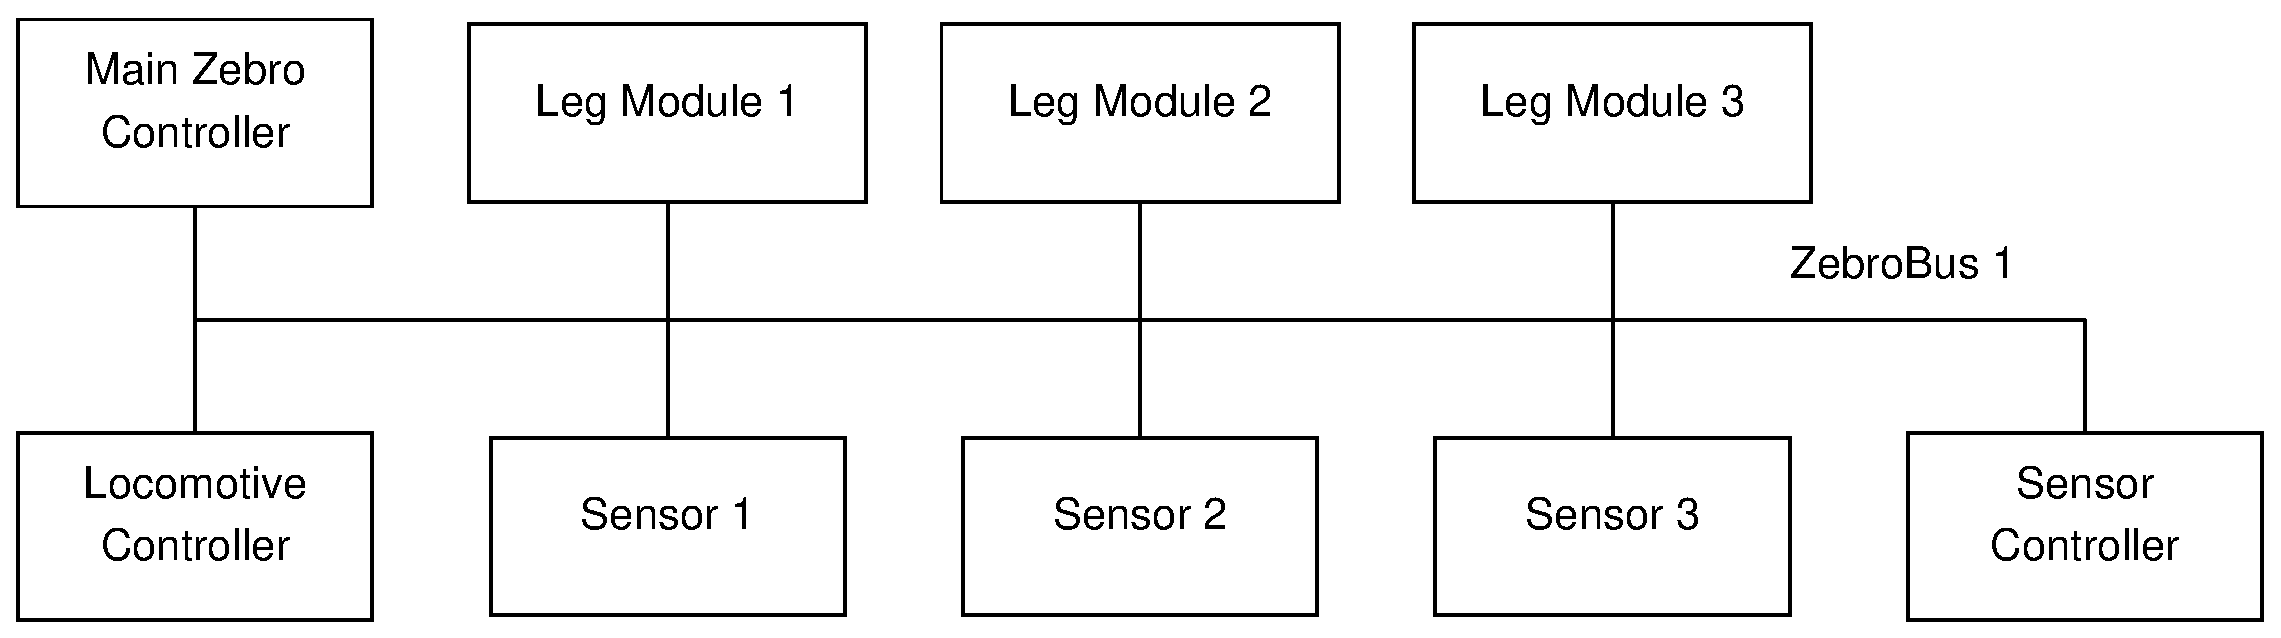
\includegraphics[scale=0.28]{fig/zebrobus_flat.eps}
                \caption{Flat hierarchy}
                \label{fig:ch3trace}     
        \end{subfigure}
        \begin{subfigure}[htpb]{\textwidth}
                \centering
                \includegraphics[scale=0.26]{fig/zebrobus_tree.eps}
                \caption{Tree hierarchy}
                \label{fig:ch3carPlotTree}
        \end{subfigure}
        \begin{subfigure}[htpb]{\textwidth}
        \centering
        \includegraphics[scale=0.28]{fig/zebrobus_mixed.eps}
        \caption{Mixed hierarchy}
         \label{fig:ch3carPlotMixed}
        \end{subfigure}
        \caption{Schematic representation of different ZebroBus hierachies.}\label{fig:zebrobus_hierachies}
\end{figure}

\subsection{Bus address space and multicast}
ZebroBus uses 7 bit bus addresses, every device on the bus should have a unique bus address.

Some data should be received by more than one module on the bus.
One approach would be to transmit it to each of these devices individually, but this has two downsides.
Firstly, more resources are used. The master has to execute the transmission multiple times, and thus the bus is occupied for a longer period of time.
Secondly, not all modules receive the data at the same time. For time sensitive data, this can be a nuisance.
Therefore, ZebroBus reserves the lowest 16 bus addresses for multicast addresses. An overview of the bus address space is given in \cref{tab:bus_address_space}. No read requests should be send to a multicast address, and all read requests received on a multicast address should be ignored.
\begin{table}[H]
    \begin{center}
    \caption{Overview of the ZebroBus bus address space.}
    \label{tab:bus_address_space}
    \begin{tabular}{ll}
    \toprule
    Address & Name \\ \midrule
    0x00 -- 0x0F & multicast addresses \\
    0x10 -- 0x6F & device addresses \\
    0x70 -- 0x7F & reserved for future use \\
    \bottomrule
    \end{tabular}
    \end{center}
\end{table}

\subsection{Virtual registers}
A common convention used with I$^2$C interfaces is that data is transferred by first transmitting the register address of the data the masters wants to read or write on the slave, followed by the actual data.
This convention was followed for ZebroBus.
Every ZebroBus device should have a set of \emph{virtual registers} or \emph{vregs}, that have the following features:

\begin{enumerate}
\item The vregs are byte addressed
\item The vregs have 256 fields
\item When reading or writing more than one byte in a single I$^2$C transaction, the read or write register address should auto increment
\item After receiving the STOP bit, the read or write register address should be reset to the address that was last received.
\item The register address is shared for read and writes. i.e. the I$^2$C sequence \\
    \verb|START 0x31 0x42 0x43 STOP START READ_BYTE STOP| should do the following:
    \begin{enumerate}
        \item Write 0x42 to register address 0x31
        \item Write 0x43 to register address 0x32
        \item Read the value in register address 0x31
    \end{enumerate}
    However, it is considered good practise to always transmit the register address before performing a read.
\end{enumerate}